% Standalone source. Main sources: 12.20.pdf pp.1--11; 12.27.pdf pp.1--6.
% The orthogonal-basis explanation and the original amplitude parameter M are restored.
\documentclass[11pt,a4paper]{article}
\usepackage[T1]{fontenc}
\usepackage{lmodern,amsmath,amssymb,booktabs,enumitem}
\usepackage[margin=22mm,headheight=14pt]{geometry}
\usepackage{tikz,fancyhdr,hyperref}
\usetikzlibrary{arrows.meta,decorations.pathmorphing,patterns}
\hypersetup{colorlinks=true,linkcolor=blue!45!black,urlcolor=blue!45!black,
  pdftitle={Mathematical Methods for Physics -- Lecture 19},pdfauthor={Zhaolong Han}}
\pagestyle{fancy}\fancyhf{}
\fancyhead[L]{\small Mathematical Methods for Physics}
\fancyhead[R]{\small Lecture 19}\fancyfoot[C]{\thepage}
\setlength{\parindent}{0pt}\setlength{\parskip}{4pt}
\setlist{topsep=3pt,itemsep=2pt,parsep=0pt}
\setlength{\emergencystretch}{1.5em}
\newcommand{\dd}{\,\mathrm{d}}
\newcommand{\R}{\mathbb{R}}
\newif\ifteachernotes\teachernotesfalse
\newcommand{\teachernote}[1]{\ifteachernotes\par\smallskip
  \noindent\textit{Instructor note.} #1\par\smallskip\fi}
\begin{document}
\begin{center}
  {\Large\bfseries Mathematical Methods for Physics---Lecture 19}\\[6pt]
  {\large Classification and Separation of Variables}\\[10pt]
  Instructor: Zhaolong Han, SOCE, Shanghai Jiao Tong University\\
  \href{mailto:han.arkey@sjtu.edu.cn}{han.arkey@sjtu.edu.cn}
\end{center}
\hrule\medskip
After classifying the basic equations, we turn from whole-line initial-value
problems to finite-interval mixed problems. We first determine the allowed
spatial modes of a string and then use the same eigenfunctions for wave, heat,
and potential equations. The interval and the boundary conditions matter at
every stage.

% Source: 12.20.pdf p.1; textbook p.300.
\section{Classification of Second-Order Equations}
Consider a linear equation in two independent variables whose principal part is
\begin{equation}
 Au_{xx}+2Bu_{xy}+Cu_{yy}+\text{lower-order terms}=f.
\end{equation}
At a point where $A,B,C$ do not all vanish, the characteristic-direction equation is
\begin{equation}
 A(\dd y)^2-2B\dd x\dd y+C(\dd x)^2=0.
\end{equation}
Its discriminant is $4(B^2-AC)$. Equivalently, use $D=B^2-AC$:
\begin{center}
\begin{tabular}{@{}lll@{}}
\toprule
Type & Criterion & Basic example\\
\midrule
Hyperbolic & $D>0$ & $u_{tt}-a^2u_{xx}=0$\\
Elliptic & $D<0$ & $u_{xx}+u_{yy}=0$\\
Parabolic & $D=0$ & $u_t-\kappa u_{xx}=0$\\
\bottomrule
\end{tabular}
\end{center}
The wave and heat examples use $(x,t)$ rather than $(x,y)$ as independent
variables. If the coefficient of $u_{xy}$ is denoted by $B$ instead of $2B$,
the corresponding discriminant is $B^2-4AC$.

% Source: 12.20.pdf pp.2--6; textbook pp.258--261.
\section{A String with Two Fixed Ends}
\subsection{Separation and the spatial eigenvalue problem}
Let $a>0$, $\ell>0$, and consider the mixed problem
\begin{equation}\label{eq:fixedproblem}
 \begin{cases}
 u_{tt}-a^2u_{xx}=0,&0<x<\ell,\ t>0,\\
 u(0,t)=u(\ell,t)=0,\\
 u(x,0)=\varphi(x),\qquad u_t(x,0)=\psi(x).
 \end{cases}
\end{equation}
Seek a nonzero separated solution $u(x,t)=X(x)T(t)$. Then
\begin{equation}
 XT''-a^2X''T=0,\qquad \frac{X''}{X}=\frac{T''}{a^2T}=-\lambda.
\end{equation}
The ratios are used where division is possible; the resulting ODEs hold also
at zeros by continuity:
\begin{equation}\label{eq:separated}
 X''+\lambda X=0,\qquad T''+a^2\lambda T=0,
 \qquad X(0)=X(\ell)=0.
\end{equation}
The spatial problem asks for the values of $\lambda$ that admit a nonzero $X$.
Such values are \emph{eigenvalues}, and the corresponding functions are
\emph{eigenfunctions}.
\teachernote{The fixed-end condition is $X(\ell)=0$. A derivative condition
 $X'(\ell)=0$ describes a different endpoint and produces a different spectrum.}

\paragraph{Case $\lambda=0$.}
Here $X=C_1+C_2x$. Both endpoint values vanish only for $C_1=C_2=0$, so zero
is not an eigenvalue for this boundary pair.

\paragraph{Case $\lambda=-\mu^2<0$.}
Write $X=C_1\cosh(\mu x)+C_2\sinh(\mu x)$. The left condition gives $C_1=0$;
the right then gives $C_2=0$ because $\sinh(\mu\ell)>0$.

\paragraph{Case $\lambda=k^2>0$.}
Now $X=C_1\cos(kx)+C_2\sin(kx)$. We obtain $C_1=0$ and
$\sin(k\ell)=0$. Therefore
\begin{equation}\label{eq:sinespectrum}
 \boxed{k_n=\frac{n\pi}{\ell},\quad \lambda_n=k_n^2,\quad
              X_n(x)=\sin(k_nx),\quad n=1,2,\ldots.}
\end{equation}
Set $\omega_n=ak_n$. The corresponding time factor is
\begin{equation}
 T_n(t)=A_n\cos(\omega_nt)+B_n\sin(\omega_nt).
\end{equation}

\begin{center}
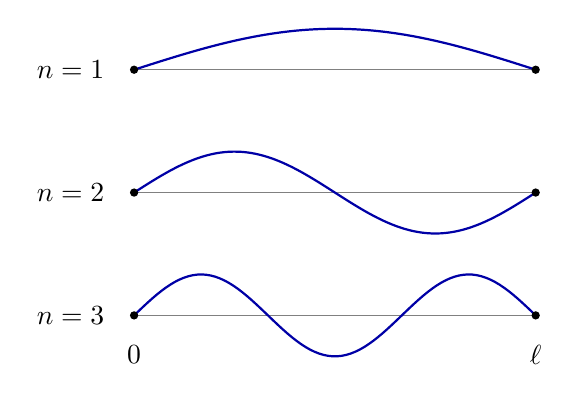
\begin{tikzpicture}[x=5.1cm,y=.52cm,>=Stealth]
 \foreach \n in {1,2,3}{
  \begin{scope}[shift={(0,{-3*(\n-1)})}]
   \draw[gray] (0,0)--(1,0);
   \draw[thick,blue!65!black,domain=0:1,samples=90]
       plot (\x,{sin(\n*180*\x)});
   \fill (0,0) circle (1.5pt);\fill (1,0) circle (1.5pt);
   \node[left] at (-.05,0) {$n=\n$};
  \end{scope}
 }
 \node[below] at (0,-6.5) {$0$};\node[below] at (1,-6.5) {$\ell$};
\end{tikzpicture}
\end{center}
Each shape satisfies the endpoint conditions, but one shape alone generally
cannot reproduce the prescribed initial displacement.

% Restores the basis statement in 12.20.pdf pp.4 and 6.
\subsection{Orthogonal basis and Fourier sine expansion}
For real functions on $(0,\ell)$, define the inner product
\begin{equation}
 \langle v,w\rangle=\int_0^\ell v(x)w(x)\dd x.
\end{equation}
The sine eigenfunctions are orthogonal:
\begin{equation}\label{eq:sineorthogonality}
 \int_0^\ell\sin(k_nx)\sin(k_mx)\dd x=
 \begin{cases}0,&n\ne m,\\ \ell/2,&n=m.\end{cases}
\end{equation}
They form a \emph{complete orthogonal basis} in $L^2(0,\ell)$. Thus a
square-integrable function can be approximated by finite sums of these modes,
with mean-square error tending to zero. This is the Fourier sine expansion.
Completeness permits the expansion; orthogonality determines its coefficients.

For example, writing
\begin{equation}
 \varphi_N(x)=\sum_{n=1}^NA_n\sin(k_nx)
\end{equation}
is analogous to resolving a vector into orthogonal directions. Multiplication
by $\sin(k_mx)$ and integration isolate $A_m$. Infinite expansions require a
convergence statement; they do not follow from linearity alone.

\subsection{Superposition and determination of coefficients}
Finite sums of the separated solutions solve the PDE and homogeneous boundary
conditions. Using the complete spatial family gives the series representation
\begin{equation}\label{eq:fixedseries}
 u(x,t)=\sum_{n=1}^\infty
       [A_n\cos(\omega_nt)+B_n\sin(\omega_nt)]\sin(k_nx).
\end{equation}
At $t=0$, the initial conditions require
\begin{equation}
 \varphi(x)=\sum_{n=1}^\infty A_n\sin(k_nx),\qquad
 \psi(x)=\sum_{n=1}^\infty\omega_nB_n\sin(k_nx).
\end{equation}
Orthogonality gives
\begin{equation}\label{eq:fixedcoefficients}
 \boxed{A_n=\frac2\ell\int_0^\ell\varphi(x)\sin(k_nx)\dd x,\qquad
 B_n=\frac2{\ell\omega_n}\int_0^\ell\psi(x)\sin(k_nx)\dd x.}
\end{equation}
The factor $1/\omega_n$ in $B_n$ comes from differentiating
$\sin(\omega_nt)$ once in time.

The procedure is a method of undetermined coefficients in a spatial orthogonal
basis: first find the eigenfunctions, then solve the time equations, and finally
use the initial data to determine their amplitudes.
For energy solutions the initial expansions are interpreted in the corresponding
integral norms. Pointwise satisfaction of the PDE requires enough regularity to
differentiate the series and satisfy the endpoint compatibility conditions.

% Source: 12.20.pdf pp.6--7. Keep M explicitly, rather than absorbing it into C.
\section{Examples for Fixed Ends}
\subsection{Example 10.1: a polynomial initial displacement}
Consider the initial data of Example 10.1 (textbook p.262):
\begin{equation}
 \varphi(x)=\frac{x(\ell-x)}M,\qquad \psi(x)=0,\qquad M>0.
\end{equation}
If an amplitude constant $C$ is used instead, it must be $C=1/M$.
We immediately have $B_n=0$. Two integrations by parts give
\begin{equation}
 \int_0^\ell x(\ell-x)\sin(k_nx)\dd x
 =\frac1{k_n}\int_0^\ell(\ell-2x)\cos(k_nx)\dd x
 =\frac{2[1-(-1)^n]}{k_n^3}.
\end{equation}
Hence
\begin{equation}
 A_n=\frac{4\ell^2}{Mn^3\pi^3}[1-(-1)^n].
\end{equation}
Even coefficients vanish, and the Fourier-series solution is
\begin{equation}
 u(x,t)=\frac{8\ell^2}{M\pi^3}\sum_{j=0}^\infty
 \frac{\cos((2j+1)\pi at/\ell)\sin((2j+1)\pi x/\ell)}{(2j+1)^3}.
\end{equation}
The odd-mode selection also reflects the symmetry of the initial shape about
$x=\ell/2$.
\teachernote{For nonzero amplitude these data have $\varphi''=-2/M$, so they do
 not satisfy the second-order corner compatibility required of a globally $C^2$
 fixed-end solution. The energy solution and the coefficient calculation remain
 valid. Second derivatives can lose continuity along characteristics from the
 initial corners; do not assert unrestricted twice-termwise differentiation.}
\emph{Regularity remark.} This example defines an energy solution; additional
corner compatibility would be needed for a globally $C^2$ classical solution.

% Source: 12.20.pdf pp.7--8.
\subsection{Initial data containing only two modes}
Take
\begin{equation}
 \varphi(x)=\sin\frac{\pi x}{\ell},\qquad
 \psi(x)=\sin\frac{4\pi x}{\ell}.
\end{equation}
Orthogonality gives $A_1=1$, $B_4=\ell/(4\pi a)$, with all other coefficients
zero. Therefore
\begin{equation}
 u(x,t)=\cos\frac{\pi at}{\ell}\sin\frac{\pi x}{\ell}
       +\frac\ell{4\pi a}\sin\frac{4\pi at}{\ell}\sin\frac{4\pi x}{\ell}.
\end{equation}
When the initial data contain finitely many eigenfunctions, the general infinite
series reduces to finitely many terms.

% Source: 12.20.pdf pp.9--11, textbook Table 10-1 and Example 10.2, p.265.
\section{How Endpoint Conditions Select the Spectrum}
\subsection{Four standard endpoint pairs}
For $X''+\lambda X=0$ on $(0,\ell)$, the positive eigenvalues are $\lambda_n=k_n^2$:
\begin{center}
\small
\begin{tabular}{@{}lll@{}}
\toprule
Endpoint conditions & $k_n$, $n\ge1$ & $X_n(x)$\\
\midrule
$X(0)=X(\ell)=0$ & $n\pi/\ell$ & $\sin(k_nx)$\\[3pt]
$X(0)=X'(\ell)=0$ & $(2n-1)\pi/(2\ell)$ & $\sin(k_nx)$\\[3pt]
$X'(0)=X(\ell)=0$ & $(2n-1)\pi/(2\ell)$ & $\cos(k_nx)$\\[3pt]
$X'(0)=X'(\ell)=0$ & $n\pi/\ell$ & $\cos(k_nx)$\\
\bottomrule
\end{tabular}
\end{center}
For the Neumann--Neumann pair there is also $\lambda_0=0$, $X_0=1$.
The squared norm is $\ell/2$ for each displayed mode and $\ell$ for $X_0$.
As an example, $X(0)=0$ removes the cosine, while $X'(\ell)=0$ requires
$\cos(k\ell)=0$, which explains the half-integer wave numbers.

\subsection{Example 10.2: one fixed and one free end}
For $u(0,t)=0$, $u_x(\ell,t)=0$, let
\begin{equation}
 \varphi(x)=3\sin\frac{3\pi x}{2\ell}+6\sin\frac{5\pi x}{2\ell},\qquad
 \psi(x)=0.
\end{equation}
These are the second and third modes of the Dirichlet--Neumann family.
Consequently,
\begin{equation}
 u(x,t)=3\cos\frac{3\pi at}{2\ell}\sin\frac{3\pi x}{2\ell}
       +6\cos\frac{5\pi at}{2\ell}\sin\frac{5\pi x}{2\ell}.
\end{equation}

% Source: 12.20.pdf p.9; 12.27.pdf pp.1--3.
\subsection{Two free ends and the zero mode}
For $u_x(0,t)=u_x(\ell,t)=0$, the expansion is
\begin{equation}
 u(x,t)=A_0+B_0t+\sum_{n=1}^\infty
       [A_n\cos(\omega_nt)+B_n\sin(\omega_nt)]\cos(k_nx),
\end{equation}
where $k_n=n\pi/\ell$ and $\omega_n=ak_n$. For $\lambda_0=0$, the time equation
is $T_0''=0$, so $T_0=A_0+B_0t$. This term must not be discarded.
The coefficients are
\begin{align}
 A_0&=\frac1\ell\int_0^\ell\varphi(x)\dd x,&
 B_0&=\frac1\ell\int_0^\ell\psi(x)\dd x,\\
 A_n&=\frac2\ell\int_0^\ell\varphi(x)\cos(k_nx)\dd x,&
 B_n&=\frac2{\ell\omega_n}\int_0^\ell\psi(x)\cos(k_nx)\dd x\quad(n\ge1).
\end{align}
The mean displacement is $A_0+B_0t$, describing uniform transverse translation.
\teachernote{In the handwritten recap, the initial-velocity coefficient line
 has a squared frequency. One time derivative produces $\omega_n$, not
 $\omega_n^2$; the formulas here agree with the earlier derivation.}

% Source: 12.27.pdf pp.3--4. kappa corresponds to the heat-equation a^2 there.
\section{The Same Spatial Modes for Heat Conduction}
For $u_t-\kappa u_{xx}=0$, separation with $X''+\lambda X=0$ gives
\begin{equation}
 T'+\kappa\lambda T=0,\qquad T_n(t)=C_ne^{-\kappa\lambda_nt}.
\end{equation}
The alternative heat coefficient $a^2$ is denoted here by $\kappa$, as in Lecture 18.
With insulated endpoints $u_x(0,t)=u_x(\ell,t)=0$,
\begin{equation}
 u(x,t)=C_0+\sum_{n=1}^\infty C_ne^{-\kappa(n\pi/\ell)^2t}
                                      \cos\frac{n\pi x}{\ell},
\end{equation}
where
\begin{equation}
 C_0=\frac1\ell\int_0^\ell\varphi(x)\dd x,\qquad
 C_n=\frac2\ell\int_0^\ell\varphi(x)\cos\frac{n\pi x}{\ell}\dd x.
\end{equation}
The zero mode is constant because $T_0'=0$. All positive modes decay.
In agreement with this,
\begin{equation}
 \frac\dd{\dd t}\int_0^\ell u(x,t)\dd x
       =\kappa[u_x(\ell,t)-u_x(0,t)]=0.
\end{equation}
The long-time temperature approaches the initial spatial average. For endpoints
held at zero temperature, use the sine family and omit the zero mode.

% Source: 12.27.pdf pp.4--6. g,h replace the source phi,psi boundary notation.
\section{Laplace's Equation in a Rectangle}
\subsection{Spatial separation and the zero mode}
Consider
\begin{equation}
 \begin{cases}
 u_{xx}+u_{yy}=0,&0<x<\ell,\ 0<y<b,\\
 u_x(0,y)=u_x(\ell,y)=0,\\
 u(x,0)=g(x),\qquad u(x,b)=h(x).
 \end{cases}
\end{equation}
\begin{center}
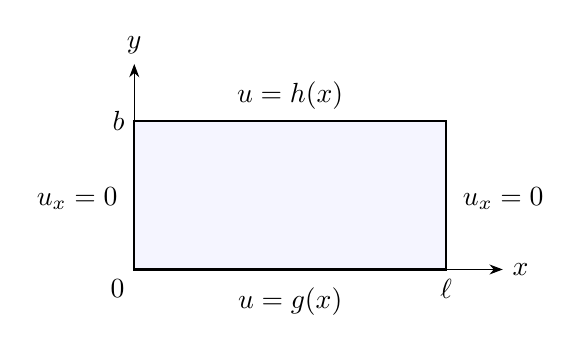
\begin{tikzpicture}[>=Stealth,scale=.9]
 \fill[blue!4] (0,0) rectangle (4.4,2.1);
 \draw[thick] (0,0) rectangle (4.4,2.1);
 \draw[->] (0,0)--(5.2,0) node[right]{$x$};
 \draw[->] (0,0)--(0,2.9) node[above]{$y$};
 \node[below left] at (0,0) {$0$};\node[below] at (4.4,0) {$\ell$};
 \node[left] at (0,2.1) {$b$};
 \node[below] at (2.2,-.12) {$u=g(x)$};
 \node[above] at (2.2,2.12) {$u=h(x)$};
 \node[left] at (-.1,1) {$u_x=0$};\node[right] at (4.5,1) {$u_x=0$};
\end{tikzpicture}
\end{center}
Put $u=X(x)Y(y)$. Then
\begin{equation}
 X''+\lambda X=0,\quad X'(0)=X'(\ell)=0,\qquad Y''-\lambda Y=0.
\end{equation}
The spatial modes are $X_0=1$ and $X_n=\cos(k_nx)$, $k_n=n\pi/\ell$.
For the remaining coordinate,
\begin{equation}
 Y_0=\alpha_0+\beta_0y,\qquad
 Y_n=\alpha_n\cosh(k_ny)+\beta_n\sinh(k_ny)\quad(n\ge1),
\end{equation}
where $\cosh z=(e^z+e^{-z})/2$ and $\sinh z=(e^z-e^{-z})/2$.
The variable in the zero mode is $y$, and $Y_0''=0$ must be solved separately.

\subsection{Matching the two remaining sides}
Define cosine coefficients for the boundary data:
\begin{align}
 g_0&=\frac1\ell\int_0^\ell g(x)\dd x,&
 h_0&=\frac1\ell\int_0^\ell h(x)\dd x,\\
 g_n&=\frac2\ell\int_0^\ell g(x)\cos(k_nx)\dd x,&
 h_n&=\frac2\ell\int_0^\ell h(x)\cos(k_nx)\dd x\quad(n\ge1).
\end{align}
Matching at $y=0$ and $y=b$ gives
\begin{equation}
 \alpha_0=g_0,\quad \beta_0=\frac{h_0-g_0}{b},\qquad
 \alpha_n=g_n,\quad
 \beta_n=\frac{h_n-g_n\cosh(k_nb)}{\sinh(k_nb)}.
\end{equation}
Thus an equivalent form of the complete solution is
\begin{align}
 u(x,y)={}&g_0\left(1-\frac yb\right)+h_0\frac yb\notag\\
 &+\sum_{n=1}^\infty\left[
  g_n\frac{\sinh(k_n(b-y))}{\sinh(k_nb)}
 +h_n\frac{\sinh(k_ny)}{\sinh(k_nb)}\right]\cos(k_nx).
\end{align}
The positive modes are harmonic and have zero $x$ derivative on the vertical
sides. The two hyperbolic-sine factors attain the lower and upper boundary
values respectively. The mean mode interpolates linearly between $g_0$ and $h_0$.
Smooth solutions up to corners require compatible boundary data; for less regular
data the boundary expansions are interpreted through their appropriate traces.

\section*{One Spatial Problem, Three Different Evolutions}
For the same spatial equation $X''+\lambda X=0$ and endpoint pair,
\begin{center}
\begin{tabular}{@{}lll@{}}
\toprule
PDE & Remaining equation & Zero-eigenvalue factor\\
\midrule
Wave & $T''+a^2\lambda T=0$ & $A_0+B_0t$\\
Heat & $T'+\kappa\lambda T=0$ & $C_0$\\
Laplace & $Y''-\lambda Y=0$ & $\alpha_0+\beta_0y$\\
\bottomrule
\end{tabular}
\end{center}
The spatial boundary conditions select the modes; the PDE determines their
time or remaining-coordinate factors; the data determine the coefficients.
The next lecture extends this procedure to nonzero boundary data and forcing.

\paragraph{Textbook pointers.}
Separation of variables: p.258 onward. Example 10.1: p.262.
Endpoint spectra and Example 10.2: Table 10-1, p.265.
Exercises: p.292, Problem 1(1)--(4) and Problem 2.

\end{document}
